\documentclass[10pt,a4paper,titlepage]{article}
\usepackage[utf8]{inputenc}     % encodage des characteres en utf8
\usepackage[francais]{babel} % pour la table des matières en français 

\usepackage{url} % pour les liens internet
\usepackage[colorlinks=true,linkcolor=black,bookmarks=true,bookmarksopen=true]{hyperref} % rendre les liens clickable
\usepackage{fancyhdr}	 
\usepackage{listings} 
\lstset{language=Java, breaklines, fontadjust, inputencoding=utf8, basicstyle=\small, numbers=left, numberstyle=\tiny, tabsize=2}

\usepackage[dvips]{graphicx}
\usepackage{epstopdf}


%%%%%%%%%%%%%%%%%%%%%%%%%%%
%   Info sur le labo
%%%%%%%%%%%%%%%%%%%%%%%%%%%
\newcommand{\branchetag}{WEB}
\newcommand{\branche}{Technologies web}
% \newcommand{\labonummer}{}
\newcommand{\laboname}{jQuery}
\newcommand{\auteurOne}{Romain de Wolff}
\newcommand{\auteurTwo}{Bruno da Silva}
\newcommand{\promo}{IL2008}

%%%%%%%%%%%%%%%%%%%%%%%%%%%


%%%%%%%%%%%%%%%%%%%%%%%%%%%%%%%%%%%%%%%%%%%%%%%%%%%%%%
% Pour l'utilisation de code
%%%%%%%%%%%%%%%%%%%%%%%%%%%%%%%%%%%%%%%%%%%%%%%%%%%%%%

\usepackage{listings} 
%\lstset{language=Java, breaklines, fontadjust, inputencoding=utf8, basicstyle=\small, numbers=left, numberstyle=\tiny, tabsize=2}

\usepackage{courier}
\usepackage{color}

% color definitions
\definecolor{dkgreen}{rgb}{0,0.6,0}
\definecolor{gray}{rgb}{0.5,0.5,0.5}
\definecolor{lightblue}{rgb}{0.92,0.92,1}

\lstset{language=Html,
  %keywords={break,case,catch,continue,else,elseif,end,for,function,
  %   global,if,otherwise,persistent,return,switch,try,while},
  keywords={script, document, function},
  basicstyle=\ttfamily\small,
  keywordstyle=\color{blue},
  commentstyle=\color{dkgreen},
  stringstyle=\color{red},
  numbers=none,
  numberstyle=\tiny\color{gray},
  stepnumber=1,
  numbersep=10pt,
  backgroundcolor=\color{lightblue},
  tabsize=2,
  linewidth=0pt,
  showspaces=false,
  showstringspaces=false,
  frame=single,
  framexleftmargin=10pt,
  framexrightmargin=10pt,
  framexbottommargin=7pt,
  framextopmargin=7pt,
  linewidth=350pt, % largeur de la ligne de code affichée
  xleftmargin=10pt, % espace avant le debut du cadre
  aboveskip=20pt
}


\pagestyle{fancy} % defini nos propre header & footer
\fancyhf{} % delete current header and footer 
\fancyhead[L]{\branchetag}
\fancyhead[C]{\laboname}
\fancyhead[R]{\auteurOne \\ \auteurTwo} 
\fancyfoot[L]{
\includegraphics[width=3cm]{img/logo-HEIG-VD.jpg}}
\fancyfoot[R]{\bfseries\thepage}

\renewcommand{\headrulewidth}{0.5pt} 
\renewcommand{\footrulewidth}{0.1pt} 
\addtolength{\footskip}{10.0pt} % space for the rule 
\fancypagestyle{plain}{
	\fancyhead{} % get rid of headers on plain pages 
	\fancyfoot{}
	\renewcommand{\headrulewidth}{0pt} % and the line 
	\renewcommand{\footrulewidth}{0pt} % and the line 
}

\author{\auteurOne, \auteurTwo}
\title{\branchetag : \laboname}
\date{\today}

\begin{document}
\pagenumbering{Roman}
\pagestyle{headings}
\begin{titlepage}
	\begin{center}
	
\includegraphics{img/logo-HEIG-VD.jpg}\\
		\vspace{3cm}
		\LARGE \branche %Laboratoire No %\labonummer \\
		\vspace{3cm}\\
		\Huge \laboname \\
		\vspace{3cm}

		\Large \textsc{Documentation Technique} \\
		\vspace{3cm}

		\large \auteurOne \\
		\auteurTwo \\	
		\vspace{10pt}
		\normalsize \textsc{\promo} \\

		\vspace{2cm}
		\today
	\end{center}
\end{titlepage}

\tableofcontents
\newpage
\pagestyle{fancy}
\pagenumbering{arabic}
\section{Introduction}


\newpage
\section{Qu'est-ce que jQuery?}
jQuery est un framework développé en javascript qui permet notamment de manipuler aisément la DOM, d'utiliser AJAX, de créer des animations...
La vocation première de ce Framework est de gagner du temps dans le développement des applications: "write less, do more".

-Pourquoi jQuery?

\newpage
\section{JavaScript et DOM}
Avant de commencer à proprement parler de jQuery, il est important d'avoir quelques notions des technologies sur lesquelles travaille jQuery. Un brève description de JavaScript et de DOM est donc nécessaire, par contre, il a été jugé inutile de présenter le HTML.

\subsection{Introduction}
A la base, le HTML est un langage totalement statique, ce qui convient pour afficher des informations statiques, mais qui devient très vite limitatif lorsqu'un contenu dynamique est désiré. C'est pour pallier à ce besoin que le Dynamic HTML (DHTML) est apparut et c'est là que l'utilisation de DOM et JavaScript devient utile.

\subsection{DOM}
% http://www.yoyodesign.org/doc/w3c/dom2-core/introduction.html
% http://fr.wikipedia.org/wiki/Document_Object_Model
Le modèle objet de document (DOM), contrairement à ce que beaucoup de personnes croient, n'est pas un langage, mais une interface de programmation d'application (API) essentiellement utilisé pour des documents HTML valides et XML bien-formés. Ce modèle (DOM), créé en 1998 par le W3C pour , définit la structure logique d'un document et la manière d'y accéder et de le manipuler. Le terme “document” est définit au un sens large par la spécification, ce qui permet par exemple à XML de stocker n'importe quel type de données sous forme de documents et ensuite de les gérer avec DOM.\\

L'API DOM permet donc de construire des documents, naviguer dans leur structure ainsi qu'ajouter, modifier ou supprimer des éléments et leur contenu. Il est ainsi possible d'accéder, modifier, supprimer ou ajouter, à quelques exceptions près, tout le contenu des documents HTML et XML.\\

Comme spécification du W3C, un objectif majeur du modèle objet document est qu'il puisse être utilisé par un grand nombre d'environnements et d'applications. Il est donc conçu de manière à pouvoir être utilisé par n'importe quel langage de programmation.\\

La structure du document DOM est très similaire à la structure des documents qu'elle modélise. Pour mieux illustrer cela, prenons l'exemple de code HTML suivant:

\begin{lstlisting}
<TABLE>
	<TBODY> 
		<TR> 
			<TD>Text1</TD>
			<TD>Text2</TD> 
		</TR> 
		<TR>
			<TD>Text3</TD>        
			<TD>Text4</TD> 
		</TR> 
	</TBODY>
</TABLE>
\end{lstlisting}

qui illustré sous forme graphique ressemble à la figure \ref{dom1}.

\begin{figure}[h]
	\begin{center}
			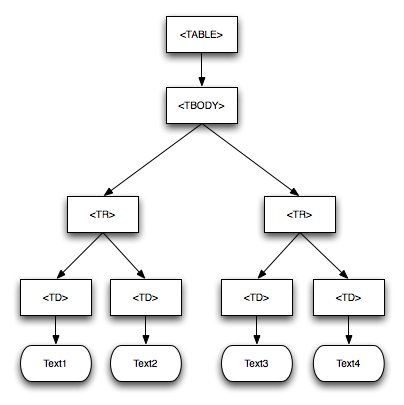
\includegraphics[width=12cm]{img/exempleDOM.png}
			\caption{Répresentation graphique DOM de l'exemple de table}
			\label{dom1}
	\end{center}
\end{figure}

On remarque que le code HTML est structure sous forme d'un arbre et que c'est très proche de la structure du code en elle-même. Ce n'est toutefois pas DOM qui spécifie cette structure en arbre, il se limite tout simplement à reproduire la structure du langage l'utilisant, qui dans ce cas est le HTML.

\subsection{JavaScript}
% http://fr.wikipedia.org/wiki/Javascript
% http://www.commentcamarche.net/javascript/jsintro.php3
JavaScript est un “langage de scripting objet” développé par Brendan Eich, aujourd'hui l'un des leaders du projet Mozilla, en 1995 chez Netscape Communications Corp. Et contrairement à ce que beaucoup de monde croit, il n'a rien à voir avec le java. Néanmoins, il possède une syntaxe similaire à ce dernier et C++ dans un souci de limiter le nombre de nouveaux concepts nécessaires à l'apprentissage du langage.\\

C'est un langage essentiellement orienté Web, qui au niveau historique se trouve être le premier langage de script pour le Web. Il a notamment permis d'apporter des améliorations au HTML en permettant d'exécuter des commandes du côté client, c'est-à-dire au niveau du navigateur et non du serveur. Il est donc fortement lié au navigateur appelant la page web incorporant le script, mais en contrepartie, il ne nécessite pas de compilateur.\\

\begin{figure}[h]
	\begin{center}
			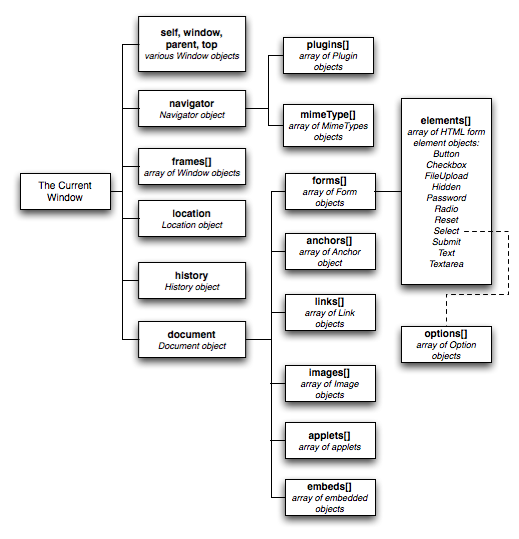
\includegraphics[width=12cm]{img/schema_js.png}
			\caption{Hiérarchie d'un objet de navigateur en JavaScript}
			\label{schema}
	\end{center}
\end{figure}

La figure \ref{schema} représente la hiérarchie d'un objet d'un navigateur en JavaScript. Ce qui permet de bien comprendre ce qu'il faut chercher et ou chercher lors de la conception d'un script.

\subsection{Qui fait quoi}
% http://developer.mozilla.org/fr/docs/Le_DOM_et_JavaScript
% 
Comme vu précédemment, le JavaScript en lui-même ne suffit pas pour accéder et modifier le contenu du code HTML. Voici donc un petit exemple qui permettra de différencier ce qui est du DOM et ce qui est du JavaScript.

\begin{lstlisting}
var anchorTags = document.getElementsByTagName("a");
for (var i = 0; i < anchorTags.length ; i++)
{
   alert("L'attribut href du " + i + "e element est : " + anchorTags[i].href + "\n");
}	
\end{lstlisting}

Dans l'exemple qui précède, les parties JavaScript sont les suivantes:
\begin{description}
	\item [\texttt{var anchorTags =}] {Création d'une variable appelée \texttt{anchorTags}}
	\item [\texttt{;}] {Fin d'instruction}
	\item [\texttt{for(var i = 0; i < }] {Boucle \texttt{for} typique dans un langage de programmation. Elle permet de parcourir chacun des noeuds de la liste \texttt{anchorTags}.}
	\item [\texttt{; i++)}] {C'est l'incrémentation de la variable \texttt{i} dans la boucle, c'est-à-dire l'incré-mentation de la boucle.}
	\item [\texttt{"L'attribut href du " + i + "e element est: " +}] {Une chaîne de caractères avec l'opérateur de concaténation (\texttt{+}).}
	\item [\texttt{"$\backslash$n");}] {Encore une fois le caractère de concaténation et une chaîne de caractères avec le caractère le retour à la ligne.}
	\item [\texttt{\}}] {Fin d'un bloc d'instructions. Dans ce cas fin de la boucle \texttt{for}.}
\end{description}

Maintenant ce qui concerne le DOM:
\begin{description}
	\item [\texttt{document.getElementsByTagName("a")}] {\texttt{document} est l'objet contenant tout ce qui se trouve sur la page. La méthode \texttt{getElementsByTagName()} renvoie une \emph{NodeList} (sorte de tableu spécifique au DOM contenant des noeuds) de toutes les balises correspondant au paramètre passé à la fonction, et ceci dans l'ordre d'apparition dans le document source. La variable \texttt{anchorsTag} est maintenant une \emph{NodeList}.}
	\item [\texttt{anchorTags.length}] {C'est la propriété \texttt{length} de l'interface \emph{NodeList}. Elle rend un entier contenant le nombre de noeuds présents dans \texttt{anchorTags}.}
	\item [\texttt{alert}] {\texttt{alert()} est une méthode DOM qui affiche une boite de dialogue avec une chaîne de caractères passée en paramètres.}
	\item [\texttt{anchorTags[i].href}] {Permet d'accéder à la propriété \texttt{href} du i\up{ème} noeud.}
\end{description}

\newpage
\renewcommand{\labelitemi}{$\bullet$}
\section{Au coeur de jQuery}
\subsection{Moteur}
-Travaille sur un objet jQuery.

\subsection{Installation \& Utilisation}\label{install}
Il est très facile d'installer jQuery. Il suffit de télécharger la librairie à l'adresse \url{http://jquery.info}, de décompresser le fichier et de le placer ou bon vous semble. Il faut ensuite insérer la ligne
\begin{lstlisting}
	<script src="lib/jquery.js" type="text/javascript\"/>
\end{lstlisting}
dans le champ \emph{head} d'un document HTML. L'attribut \texttt{src="lib/jquery.js"} correspond au chemin vers la librairie jQuery, qui dans cet exemple est placée dans un répertoire \texttt{lib} se trouvant dans le même répertoire que le fichier HTML.\\

Une fois ceci fait, la libraire est prête à être utilisée en appelant simplement les méthodes existantes de la librairie.

\begin{lstlisting}
<html>
	<head>
		<script type="text/javascript" src="jquery-1.2.1.js"/>
		<script>
			$(document).ready(function() {		
				$("a.lien").click(function() {
					$("p.text").toggle(150);
				});
			});
		</script>
	</head>
	<body>

		<a href="#" class="lien">anim: toggle()</a>

	<p class="text" style="border:1px solid black; color: green;">
		<br>Teste avec jQuery<br><br></p>
		
	</body>
</html>
\end{lstlisting}

L'exemple ci-dessus montre comment utiliser importer la librairie jQuery et ensuite d'appeler la méthode \texttt{toggle()} qui cache ou affiche les liens référencés respectivement s'ils sont visibles ou cachés. Cette méthode est appelée lorsqu'un click est détecté et c'est la méthode \texttt{click()} qui le fait. Ces deux méthodes sont toutes les deux issues de la librairie jQuery.

\subsection{Librairie}
Comme expliqué au chapitre \ref{install}, l'appel à un simple fichier suffit pour pouvoir utiliser la librairie et à l'instar d'un langage comme Java, jQuery ne possède actuellement qu'une seule librairie. Néanmoins, il est possible de catégoriser les différentes méthodes afin de pouvoir mieux s'y retrouver lors d'une recherche.\\

C'est exactement qui a été fait dans la documentation officielle et par l'excellente traduction française respectivement disponibles aux adresses \url{http://docs.jquery.com/Main_Page} et \url{http://jquery.developpeur-web2.com/}.\\

C'est donc également par catégories que la librairie sera décrite dans ce document. Néanmoins, cette description est faite dans le but d'informer de certaines possibilités existantes et ne sera pas exhaustive. Donc pour des informations plus précises, il faut se référer aux deux sites cités ci-dessus.

\subsubsection{Fonctions essentielles}
Cette partie de la librairie met à disposition ce que les concepteurs ont estimé être les fonctions de base pour pouvoir faire du jQuery. En effet, c'est là qu'il est possible de trouver les fonctions construisant un objet jQuery et ensuite d'exécuter dessus certaines opérations:

\begin{itemize}
	\item parcourir tous les éléments de l'objet et appliquer un traitement dessus;
	\item chercher des éléments par position;
	\item trouver la position d'un élément;
	\item savoir combien de combien d'éléments est composé l'objet.\\
\end{itemize}

Voici un petit exemple pour mieux illustrer cela:

\begin{lstlisting}
$("img").each(function(i){
	this.src = "test" +  i +  ".jpg";
});
\end{lstlisting}

Le code ci-dessus créé un objet jQuery contenant tous les éléments \texttt{img} de la page web, les parcourt et ajoute la source de l'image.\\

Code de test:
\begin{lstlisting}
<img/><img/>
\end{lstlisting}


Résultat:
\begin{lstlisting}
<img src="test0.jpg"/><img src="test1.jpg"/>
\end{lstlisting}

\subsubsection{Attributs}
Cette partie regroupe les fonctions permettant d'accéder aux attributs des balises HTML. Elles permettent entre autres d'ajouter, modifier ou supprimer la valeur de l'attribut. Elles permettent également d'insérer ou supprimer un attribut.\\

Par exemple, le code qui suit permet d'ajouter l'attribut \texttt{src} avec la valeur \texttt{test.jpg} à la balise \texttt{img}.

\begin{lstlisting}
$("img").attr("src","test.jpg");
\end{lstlisting}


Code de test:
\begin{lstlisting}
<img/>
\end{lstlisting}


Résultat:
\begin{lstlisting}
<img src="test.jpg"/>
\end{lstlisting}

\subsubsection{Parcours}
Cet ensemble est divisé en deux types de fonctions:
\begin{itemize}
	\item filtre;
	\item recherche.\\
\end{itemize}

Le premier type de la liste permet, comme son nom l'indique, de faire un filtrage sur l'objet jQuery, ce qui veut dire effectuer un tri parmi l'objet. L'exemple qui suit parcourt tout l'objet et retourne tous les éléments appartenant à la classe \texttt{selected}.

\begin{lstlisting}
$("p").filter(".selected")
\end{lstlisting}

Code de test:
\begin{lstlisting}
<p class="selected">Hello</p><p>How are you?</p>
\end{lstlisting}

Résultat:
\begin{lstlisting}
[ <p class="selected">Hello</p> ]
\end{lstlisting}

Le deuxième type de la liste permet d'effectuer des recherches dans l'objet jQuery. L'exemple suivant permet de rechercher tous les enfants de chaque \texttt{div}.

\begin{lstlisting}
$("div").children()
\end{lstlisting}


Code de test:
\begin{lstlisting}
<p>Hello</p><div>Hello Again</div><p>And Again</p>
\end{lstlisting}


Résultat:
\begin{lstlisting}
[Hello Again]
\end{lstlisting}

\subsubsection{Manipulation}
Les fonctions de type manipulation permettent de changer, remplacer, supprimer ou copier le contenu. Permettent également l'insertion au milieu, avant, après, autour.\\

L'exemple suivant p

\subsubsection{CSS}
\subsubsection{Evénements}
\subsubsection{Effets}
\subsubsection{AJAX}
\subsubsection{Fonctions diverses}
\subsubsection{UI}

\subsection{Compatibilité avec les navigateurs}
% http://docs.jquery.com/Browser_Compatibility
La version actuelle de jQuery est supportée par les navigateurs suivants:

\begin{itemize}
	\item {Firefox 1.5+;}
	\item {Internet Explorer 6+;}
	\item {Safari 2.0.2+;}
	\item {Opera 9+.\\}
\end{itemize}

Par contre, certains problèmes ont été reportés sur les suivantes versions:
\begin{itemize}
	\item {Firefox 1.0.x;}
	\item {Internet Explorers 1-5.x;}
	\item {Safari 1.x;}
	\item {Safari 2.0;}
	\item {Opera 1.0-8.5;}
	\item {Konqueror.\\}
\end{itemize}

En général, jQuery fonctionne avec Konqueror et Firefox 1.0.x, mais il peut se produire certains bugs depuis que les tests ne sont pas fait aussi régulièrement qu'avec les versions plus récentes.\\

Pour des renseignements plus précis sur la compatibilité d'un navigateur en particulier, il existe un très bon test à l'adresse \url{http://jquery.com/test/}.

\newpage
\section{Comparatif}

\newpage
\section{Conclusion}

% \appendix
% 
% \newpage
% \section{CACMIndexer.java}
% \lstinputlisting{../src/rim/cacm/CACMIndexer.java}
% 
% \newpage
% \section{CACMRetriever.java}
% \lstinputlisting{../src/rim/cacm/CACMRetriever.java}

\end{document}